\chapter{Teoria da informação em análise de formas}

Neste capítulo apresentamos como  grandezas e medidas da teoria da informação podem ser utilizadas na descrição e na avaliação de similaridade de formas.

Iniciamos o capítulo apresentando a entropia de Shannon, a entropia diferencial e suas propriedades. 

Em seguida descrevemos a metodologia utilizada para obtenção de descritores de forma a partir dessas entropias.



\section{Entropia como descritor multiescala}

No capítulo \ref{chap:contour} mostramos como se obtém a curvatura multiescala como uma assinatura do contorno de uma forma. No mesmo capítulo apresentamos um descritor multiescala construído a partir da versão discreta dessa assinatura, mais especificamente a energia de dobramento multiescala. 

Aqui propomos dois novos descritores multiescala construídos a partir dessa mesma assinatura, mas explorando os conceitos de entropia discreta de Shannon e de entropia diferencial.

Para se obter tais descritores é necessário estimar as funções densidade de probabilidade do sinal da curvatura em diferentes escalas. No caso da entropia de Shannon, que tem em sua definição uma função densidade de probabilidade de massa, a maneira mais direta de se realizar tais estimativas é através de histogramas. Já no caso da entropia diferencial, empregamos para realizar tais estimativas o método da janela de Parzen.

\subsection{Entropia discreta da curvatura multiescala}

Sendo  $K[t,\sigma]$ a função curvatura multiescala do contorno de uma forma, discretizada em $M$ pontos e $U$ escalas, temos $\sigma = \{\sigma_1\text{, }\sigma_2\text{, }\ldots\text{, }\sigma_U\}$ como sendo os fatores de escala e $t = \{1\text{, }2\text{, }\ldots\text{, }M\}$ os índices dos possíveis valores da curvatura ao longo do perímetro do contorno. Fixada uma escala $\sigma'$ obtemos o histograma dessa função subdividindo o intervalo dos valores que a função curvatura multiescala pode assumir em $N$ faixas distintas de mesmo tamanho $\Delta x$ e contando o número de ocorrências dos valores dessa função dentro de cada uma dessas faixas  \cite{Webb:2002}. Desta forma, o valor de $\Delta x$ será   

\begin{equation}
\Delta x = \frac{\max\limits_{\forall t}{K[t,\sigma']}-\min\limits_{\forall t}{K[t,\sigma']}}{N}\text{,}
\end{equation}

 sendo o histograma

\begin{equation}\label{eq:histograma}
P\big(K[t,\sigma']\big) = \Big\{P_j|\:j = 1\text{, }2\text{, }\ldots\text{, }N\Big\}\text{, }
\end{equation}

%\begin{equation}
%P_\sigma[j] = \frac{n_j}{\sum\limits_{i=1}^Nn_i}\text{,}
%\end{equation}

 com $P_j=\frac{n_j}{\sum\limits_{i=1}^Nn_i}$ e $n_j = \#\{x \in \Re|\:\min\limits_{\forall t}{\big(K[t,\sigma']\big)}- j\Delta x \leq x \leq \min\limits_{\forall t}{\big(K[t,\sigma']\big)}+j\Delta x\}$. O operador $\#A$ denota a cardinalidade do conjunto A. 
 
 A entropia discreta da curvatura multiescala é obtida aplicando-se a equação \ref{eq:Shannon} ao histograma da função curvatura, obtido através da equação \ref{eq:histograma}, para os diferentes fatores de escala. Temos assim o descritor entropia discreta da curvatura multiescala como sendo
 
\begin{equation}
EDM = \big(H_{\sigma_1}\text{, } H_{\sigma_2}\text{, }\ldots\text{, }H_{\sigma_U}\big)
\end{equation}

aonde $H_{\sigma_u} = H(P_{\sigma_u})$ e $P_{\sigma_u} = P\big(K[t,\sigma_u]\big)$.
 
\subsection{Entropia diferencial da curvatura multiescala}

O cálculo da entropia diferencial da curvatura multiescala, através da equação \ref{eq:difent}, requer que se estime as funções densidade de probabilidade do sinal da curvatura em diferentes escalas.  A técnica não paramétrica da janela de Parzen pode ser utilizada para realizar tais estimativas. 
 
 Para uma dada escala $\sigma'$, temos a curvatura amostrada em $M$ valores como sendo $K[t,\sigma'] = \{K[1,\sigma']\text{, }K[2,\sigma']\text{, }\ldots\text{, }K[M,\sigma']\}$. A função densidade de probabilidade dessa função, estimada pela janela de Parzen, é dada por \cite{Webb:2002}:  
 
\begin{equation}\label{eq:parzen}
p_{\sigma'}(k) = \frac{1}{bM}\sum\limits_{i=1}^M\Psi(\frac{k - K[i,\sigma']}{b})\text{,}
\end{equation}

sendo $\Psi(z) = \frac{1}{\sqrt{2\pi}}\exp{-\frac{z^2}{2}}$ a função de janela e $b$ a sua largura de banda.

No processo de estimação através dessa técnica a escolha do parâmetro largura de banda é crítica, pois esse altera o grau de suavização da curva de densidade obtida. Valores elevados desse parâmetro tendem a suavizar em demasia a curva de densidade estimada acarretando em perda de detalhes importantes. Por outro lado, valores pequenos resultam em densidades estimadas com mais detalhes, porém mais ruidosa. Assim, é importante estabelecer um critério para escolha do parâmetro de largura de banda para que se tenha uma boa estimativa da função densidade de probabilidade. Adotamos neste trabalho o método proposto por Silverman \cite{silverman:1986}. Esse método, que determina uma escolha ótima de largura de banda, assume que a distribuição de probabilidade dos dados é normal e que a janela utilizada é gaussiana.

A largura de banda pelo método de Silverman é dada por \cite{silverman:1986}

\begin{equation}
b = \big(\frac{4\hat{\sigma}^5}{3n}\big)^\frac{1}{5}\text{,}
\end{equation}

sendo $\hat{\sigma}$ o desvio padrão e $n$ o número das amostras utilizadas no processo de estimação. 

Temos o cálculo da entropia diferencial da curvatura multiescala na escala $\sigma'$ aplicando o resultado obtido da equação \ref{eq:parzen} na equação \ref{eq:difent}, ou seja:

\begin{equation}\label{eq:desc_entropia}
h\big(K[t,\sigma']\big) = -\int_{-K_{min}}^{K_{max}}p_{\sigma'}(k)\log{p_{\sigma'}(k)}dk\text{, }
\end{equation}

sendo a integral calculada através do método numérico de integração de Simpson e os limites de integração $K_{min}$ e $K_{max}$ os valores máximos e mínimos da curvatura multiescala na escala $\sigma'$.

O descritor obtido a partir da equação \ref{eq:desc_entropia} apresenta propriedades de invariância a translação e a rotação. Isso porque a translação da forma não afeta o sinal da curvatura. Embora a rotação desloque em fase o sinal da curvatura, como ilustra a figura \ref{fig:curv_scale_rot}a, esse deslocamento não interfere na função densidade de probabilidade estimada, e portanto não interfere no cálculo do descritor.

Porém, o descritor não apresenta invariância a mudança de escala da forma. Isso porque tal mudança reflete em escala no sinal de curvatura (figura \ref{fig:curv_scale_rot}b), o que interfere na função densidade de probabilidade estimada, e portanto no cálculo do descritor.

Consegue-se a invariância do descritor à mudança de escala utilizando o perímetro da forma ($L_{\sigma'}$) como fator de normalização. Desta forma, aplicando a  propriedade da equação \ref{eq:escala_entropia}, temos a versão do descritor invariante a mudança de escala:

\begin{equation}\label{eq:entropia_inv}
\hat{h}\big(K(t,\sigma')\big) = -\int_{-K_{min}}^{K_{max}} p_{\sigma'}(k)\log{p_{\sigma'}(k)}dk+\log{L_{\sigma'}}\text{.}
\end{equation}

\begin{figure}[]
\caption{\label{fig:curv_scale_rot}Efeitos da rotação e da mudança de escala das formas sobre a curvatura.}
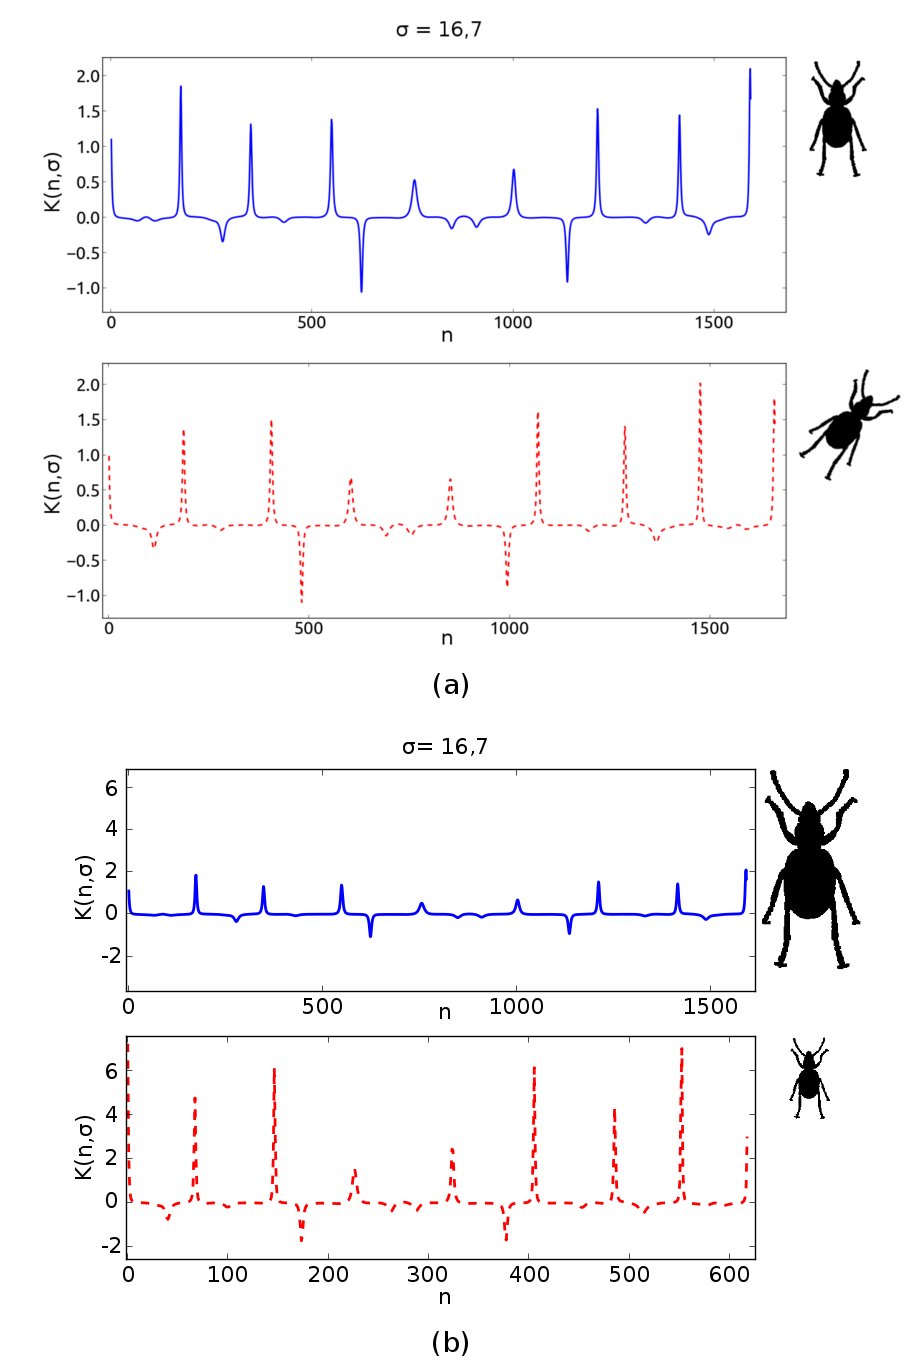
\includegraphics[width=\textwidth]{curvatura_scale_rot.png}
\legend{Fonte: próprio autor.}
\end{figure}

As figuras \ref{fig:entropia_inv}a e \ref{fig:entropia_inv}b ilustram o descritor entropia diferencial da curvatura multiescala, calculado para duas formas idênticas, em diferentes escalas. Na figura \ref{fig:entropia_inv}a o cálculo foi realizado através da equação \ref{eq:entropia_inv} e o descritor mostrou invariância à mudança de escala da forma. Já na figura \ref{fig:entropia_inv}b o cálculo foi realizado a partir da equação \ref{eq:desc_entropia} e o descritor não apresentou invariância à escala da forma.

A figura \ref{fig:entropia_inv}c ilustra a invariância do descritor à rotação da forma. Nesse caso, o cálculo foi realizado a partir da equação \ref{eq:entropia_inv}.

\begin{figure}[]
\caption{\label{fig:entropia_inv}Efeitos da rotação e da mudança de escala das formas sobre o descritor entropia diferencial da curvatura multiescala.}
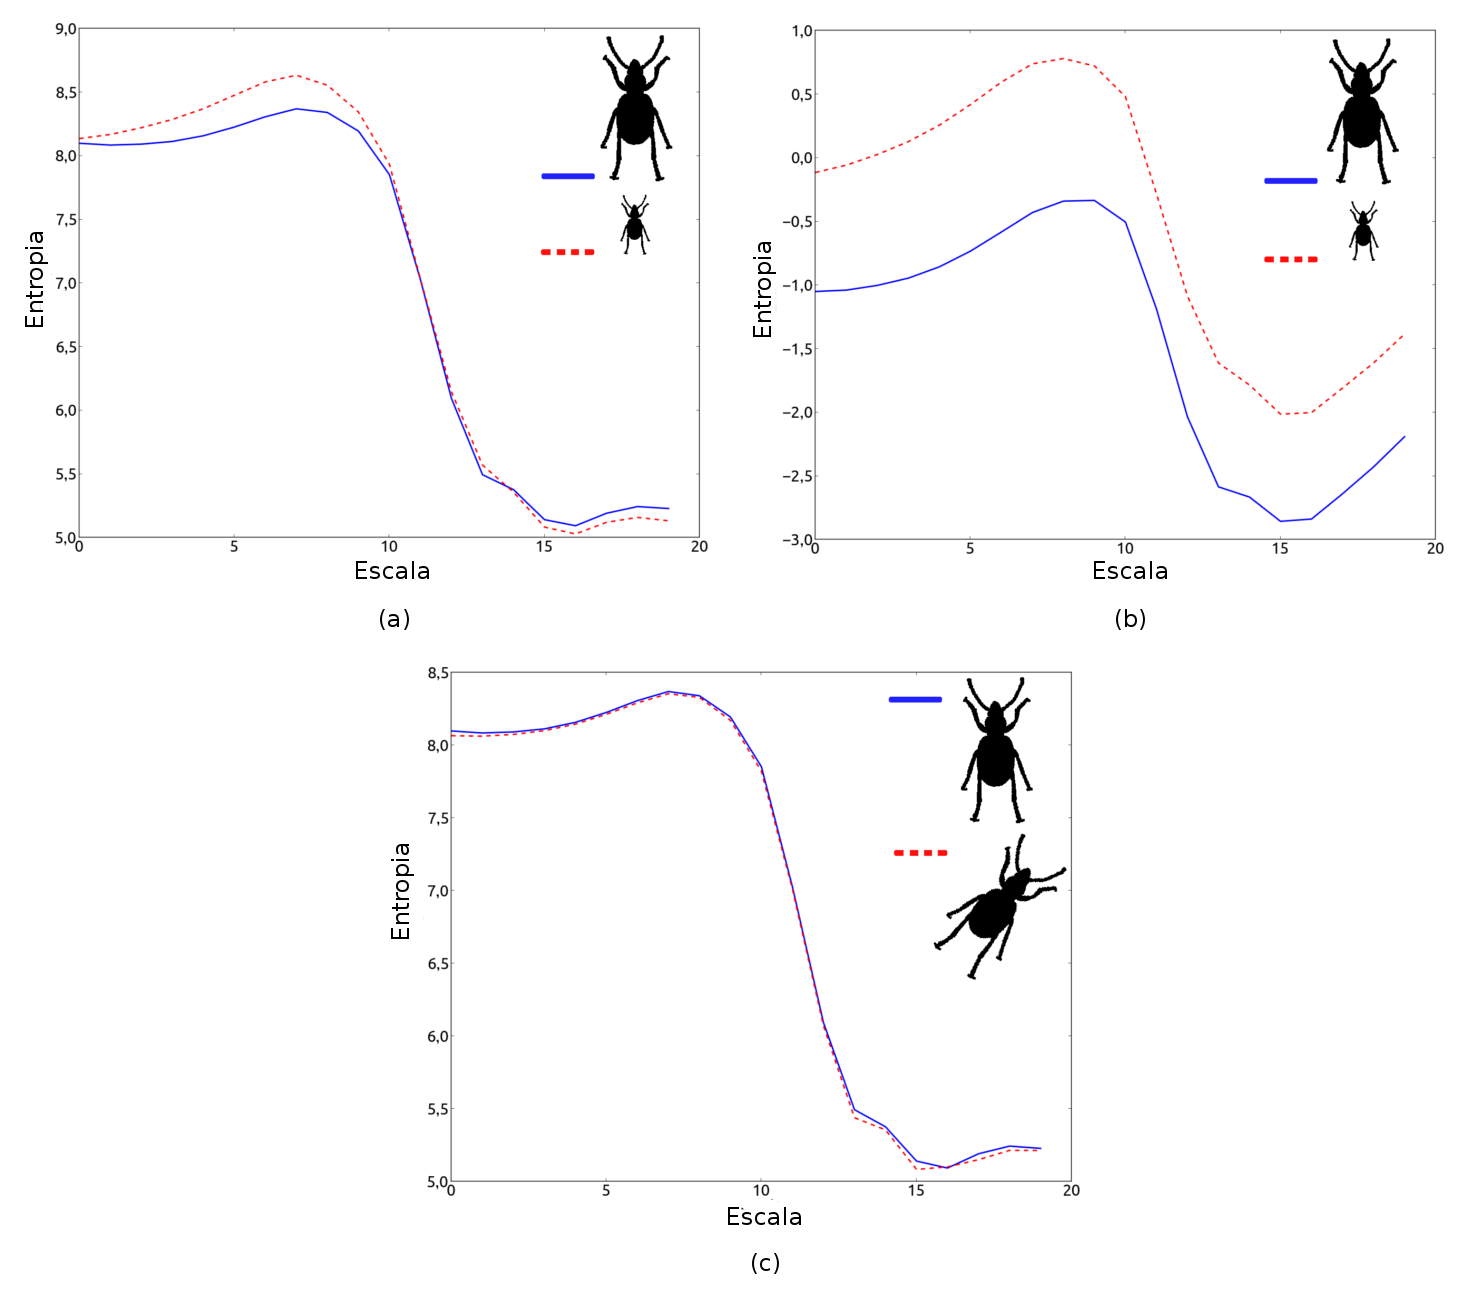
\includegraphics[width=\textwidth]{inv_entropia.png}
\legend{Fonte: próprio autor.}
\end{figure}

\section{Medidas de divergência em avaliação de similaridade de formas}

%Um desses conceitos é o de divergência estocástica.

A avaliação de similaridade entre formas a partir de medidas de divergência requer que as informações das assinaturas, abordadas na Seção \ref{sec:Assinatura} do Capítulo \ref{chap:contour}, sejam tratadas como variáveis aleatórias e que suas distribuições de probabilidade sejam estimadas. 

Está ilustrado na  Figura \ref{fig:metodo_distancia} como divergentes podem ser aplicados na avaliação da similaridade entre duas formas A e B. No método em questão, as distribuições de probabilidade de quatro assinaturas distintas dos contornos das formas são estimadas, através de histogramas, para em seguida se calcular as medidas de divergência. 

Uma medida de similaridade é então obtida  a partir da média ponderada das medidas de divergência.

\begin{figure}[h!]
  \caption{\label{fig:metodo_distancia} Método para avaliação da similaridade entre duas formas A e B utilizando distância estocástica e histogramas das assinaturas do contorno das formas.}
  \centering
  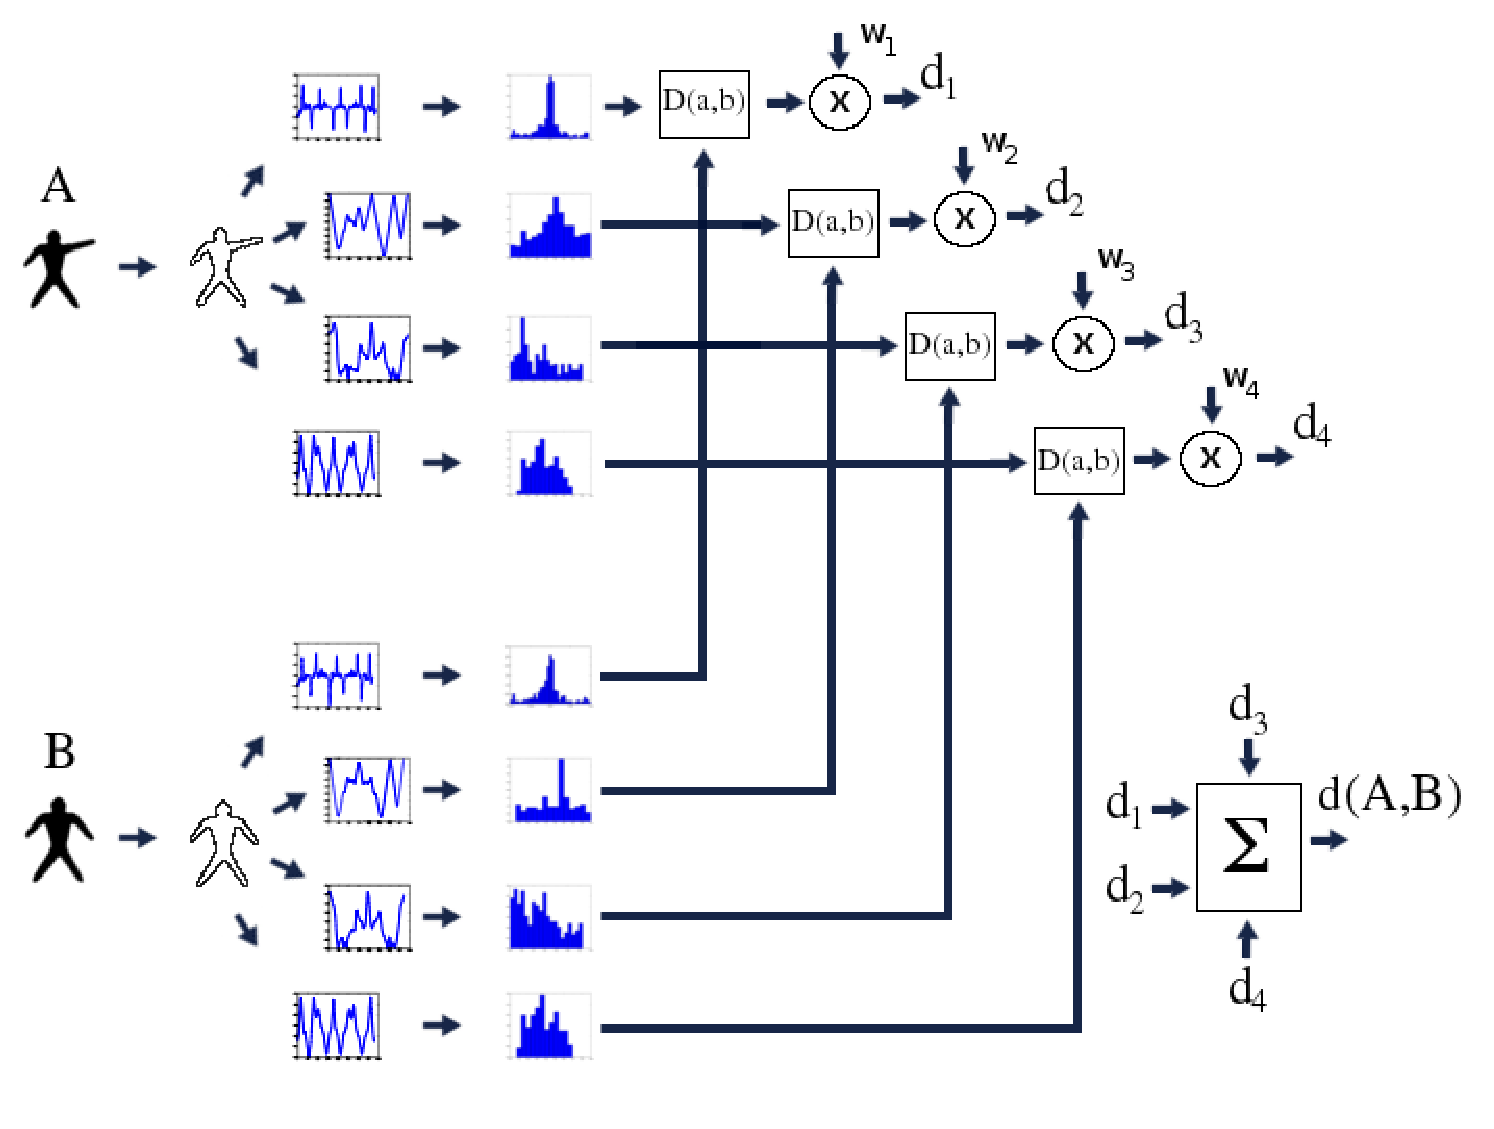
\includegraphics[width=0.85\textwidth]{figura_metodo.eps}
\end{figure}


\section{Metodologia de avaliação de desempenho}

\subsection{Experimentos CBIR}
Os experimentos de recuperação de imagens pelo conteúdo que realizamos visam avaliar o desempenho dos descritores de formas e das medidas de similaridade estudadas neste trabalho. As metodologias utilizadas nesses experimentos são as mesmas encontradas em diversos trabalhos de recuperação de formas da literatura.

São empregadas nos experimentos duas bases de imagens de formas binárias: a Kimia, de 99 formas, e a MPEG-7 CE-Shape-1 de 1400 formas. Ambas as bases estão apresentadas no Apêndice deste trabalho.

A Figura \ref{fig:metodo_cbir} ilustra a metodologia dos experimentos. Primeiramente realiza-se a extração de características das formas da base de imagens de formas binárias com o método de descrição sob avaliação. O mesmo processo de extração de características é aplicado a imagem de uma forma de consulta. Esse processo resulta numa base de dados com os vetores de características associados às formas utilizadas no experimento. 

Com a medida de similaridade avalia-se o grau de correspondência existente entre o vetor de características da forma de consulta e os vetores associados a cada uma das formas da base. Tem-se assim como resultado uma lista de imagens recuperadas em ordem decrescente de similaridade à forma de consulta. Todo esse processo é realizado repetidamente tomando-se cada forma da base de imagens como forma de consulta e recuperando-se as demais.

\begin{figure}[h!]
  \caption{\label{fig:metodo_cbir} Metodologia empregada para os experimentos de recuperação de formas pelo conteúdo.}
  \centering
  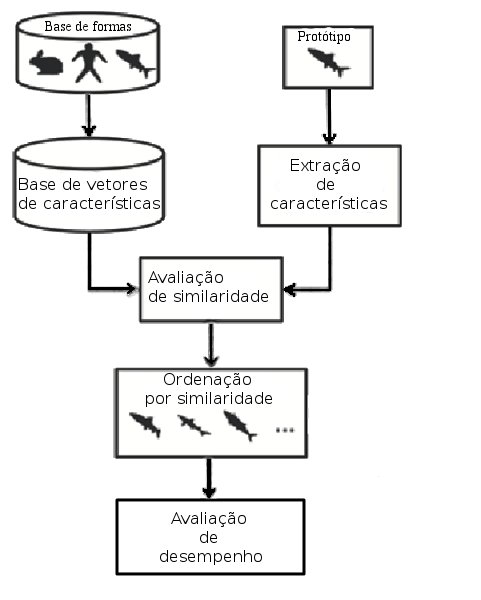
\includegraphics[width=0.55\textwidth]{Metodologia1.jpg}
\end{figure}

Na avaliação do desempenho dos experimentos duas medidas são utilizadas: o número total de acertos por posição recuperada e a medida Bull-eye.

A primeira medida consiste no número total de ocorrências de formas da mesma classe que a forma de consulta em cada posição recuperada. Um exemplo que ilustra o processo de cálculo dessa medida está apresentado na figura \ref{fig:ex_metodo_cbir}. Nesse exemplo foram realizados quatro experimentos de recuperação de formas, sendo apresentado como resultado de cada experimento as onze formas mais similares à forma de consulta. As posições aonde as formas estão destacadas em vermelho correspondem àquelas aonde a recuperação não foi correta e as demais posições, aonde não há destaque, correspondem àquelas aonde as formas foram recuperadas corretamente. Na última linha temos a medida de avaliação de desempenho. Observe que, nesse exemplo, essa é formada por onze colunas, sendo o valor em cada coluna a soma do número total de acertos dos experimentos de recuperação em cada posição correspondente.

Em alguns trabalhos de recuperação de formas pelo conteúdo, o número total de acertos por posição recuperada é calculado para a base Kimia-99 \cite{Bernier:2003}. Tendo esta base 99 formas, igualmente distribuídas em 9 classes, são realizadas 99 recuperações das 11 formas mais similares à imagem de consulta. Como resultado espera-se obter um total de 99 formas recuperadas corretamente para cada posição recuperada.

\begin{figure}[h!]
  \caption{\label{fig:ex_metodo_cbir} Exemplo ilustrando um experimento de recuperação de formas e o cálculo do número total de acertos por posição recuperada}
  \centering
  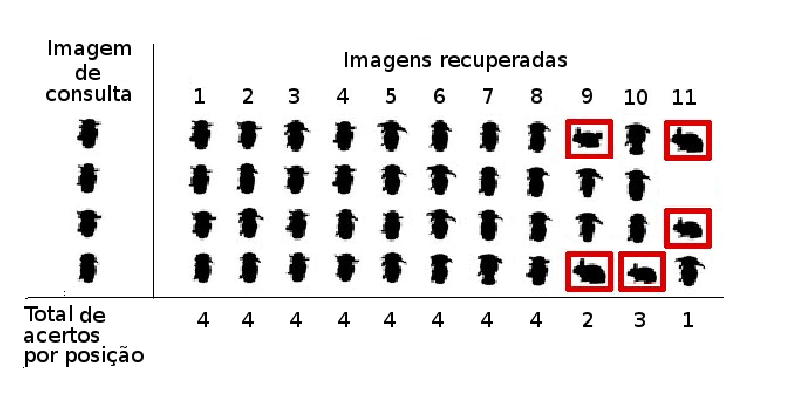
\includegraphics[width=0.75\textwidth]{ex_retrieval.eps}
\end{figure}

A medida Bull-eye também é utilizada na literatura para a comparação de diferentes métodos de recuperação de formas. Essa medida é calculada para a base MPEG-7 CE-Shape-1 da seguinte maneira: tomando-se cada forma dessa base de imagens como elemento de consulta, contabiliza-se o número de recuperações pertencentes a mesma classe da forma de consulta dentre as 40 primeiras posições recuperadas. Como resultado calcula-se a percentagem da quantidade máxima de recuperações corretas possíveis de se alcançar, sendo esta última quantidade $28000 = 1400\text{ formas} \times 20\text{ recuperações corretas poro forma}$. 

\subsection{Visualizaçâo de dados}

A Figura \ref{fig:metodo_4} ilustra o método que empregamos na avaliação da capacidade discriminativa dos descritores de formas através das técnicas de visualização dos dados apresentadas.

\begin{figure}[h!]
  \caption{\label{fig:metodo_4} Método de avaliação de descritores multiescala do contorno de formas. (a) Base de imagens. (b) Extração de características. (c) Descritores de formas. (d) Análise de similaridade a partir da matriz-U. (e) Avaliação de agrupamentos a partir da medida silhouette.}
  \centering
  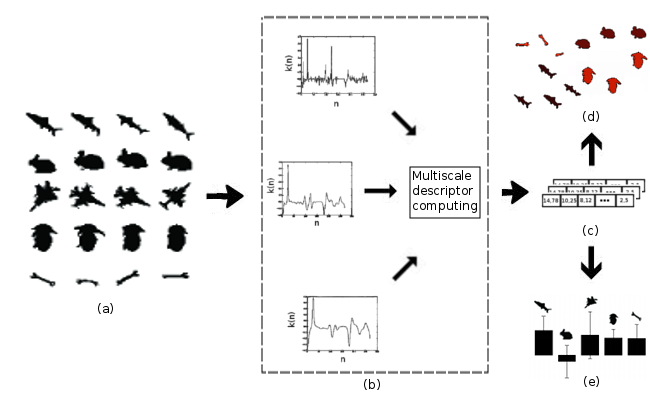
\includegraphics[width=0.75\textwidth]{metodo_v4.png}
\end{figure}

O primeiro passo consiste em realizar a extração de características num conjunto de formas binárias rotuladas (Figura \ref{fig:metodo_4}a e Figura \ref{fig:metodo_4}b) com o método de descrição sob análise. Como resultado temos um conjunto de descritores, ou vetores de características, das referidas formas (Figura \ref{fig:metodo_4}c). 

A avaliação de qualidade dos descritores se dá qualitativamente e quantitativamente. Na avaliação qualitativa (Figura \ref{fig:metodo_4}d) utilizamos a rede auto-organizável de Kohonen para obtenção da matriz de distâncias unificada, ou matriz-U. Essa última é empregada como ferramenta de visualização dos dados, o que possibilita identificar como o método de descrição sob avaliação agrupa as formas. 

Na avaliação quantitativa (Figura \ref{fig:metodo_4}e) utilizamos os rótulos e os vetores de características das formas para calculamos a medida de avaliação de agrupamentos \emph{Silhouette} \cite{Rousseeuw:1987}. Valores médios dessa medida, por classe de formas, indica a habilidade dos descritores em discriminar formas que pertençam a classes distintas e de agrupar formas que pertençam a uma mesma classe.
\begin{comment}

\section{Fusão de características}

Conforme ilustra a Figura \ref{fig:features1} contruímos três bases de dados de vetores de características multiescala a partir das formas da base da Figura \ref{fig:db1}. A aplicação da técnica PCA às características multiescala possibilita obter como saída vetores de componentes descorrelacionadas e de máxima variância (citar). 

\begin{figure}[h!]
  \caption{\label{fig:features1} Metodologia que emprega a técnicas \emph{PCA} para obtenção de um descritor híbrido através da fusão de descritores multiescala.}
  \centering
  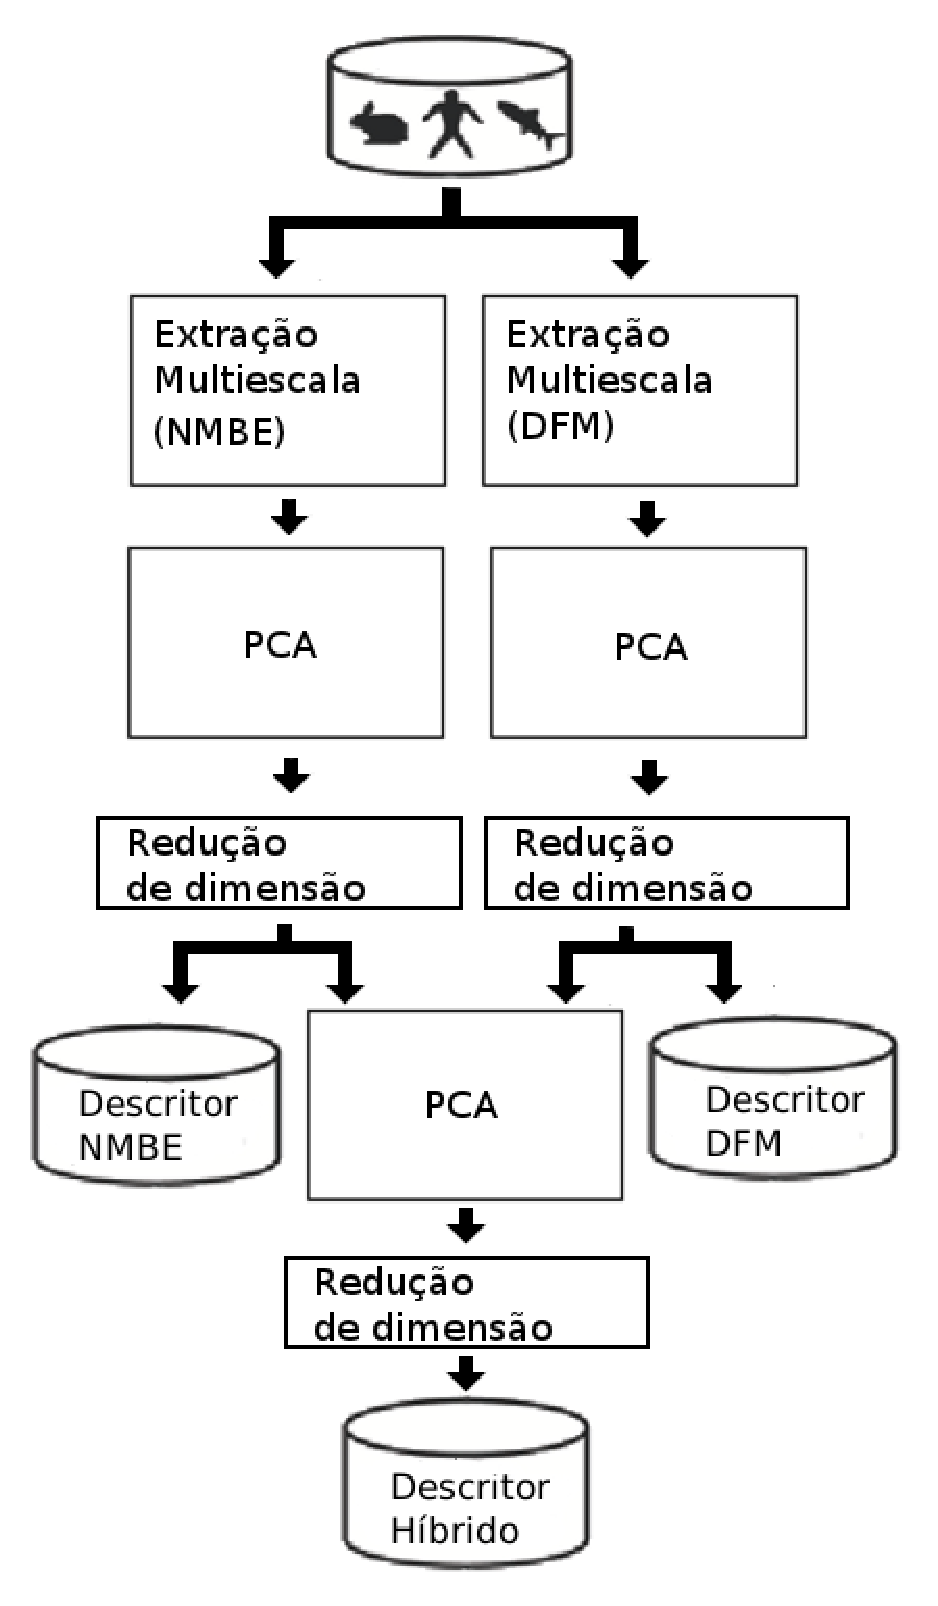
\includegraphics[width=0.45\textwidth]{features1.eps}
\end{figure}

\begin{figure}[h!]
  \caption{\label{fig:acuracia} Acurácia média por classe aferida nos experimentos de recuperação de formas pelo conteúdo, com a base Kimia-99, para os descritores (a) Dimensão fractal multiescala; (b) Energia de dobramento multiescala.}
  \centering
  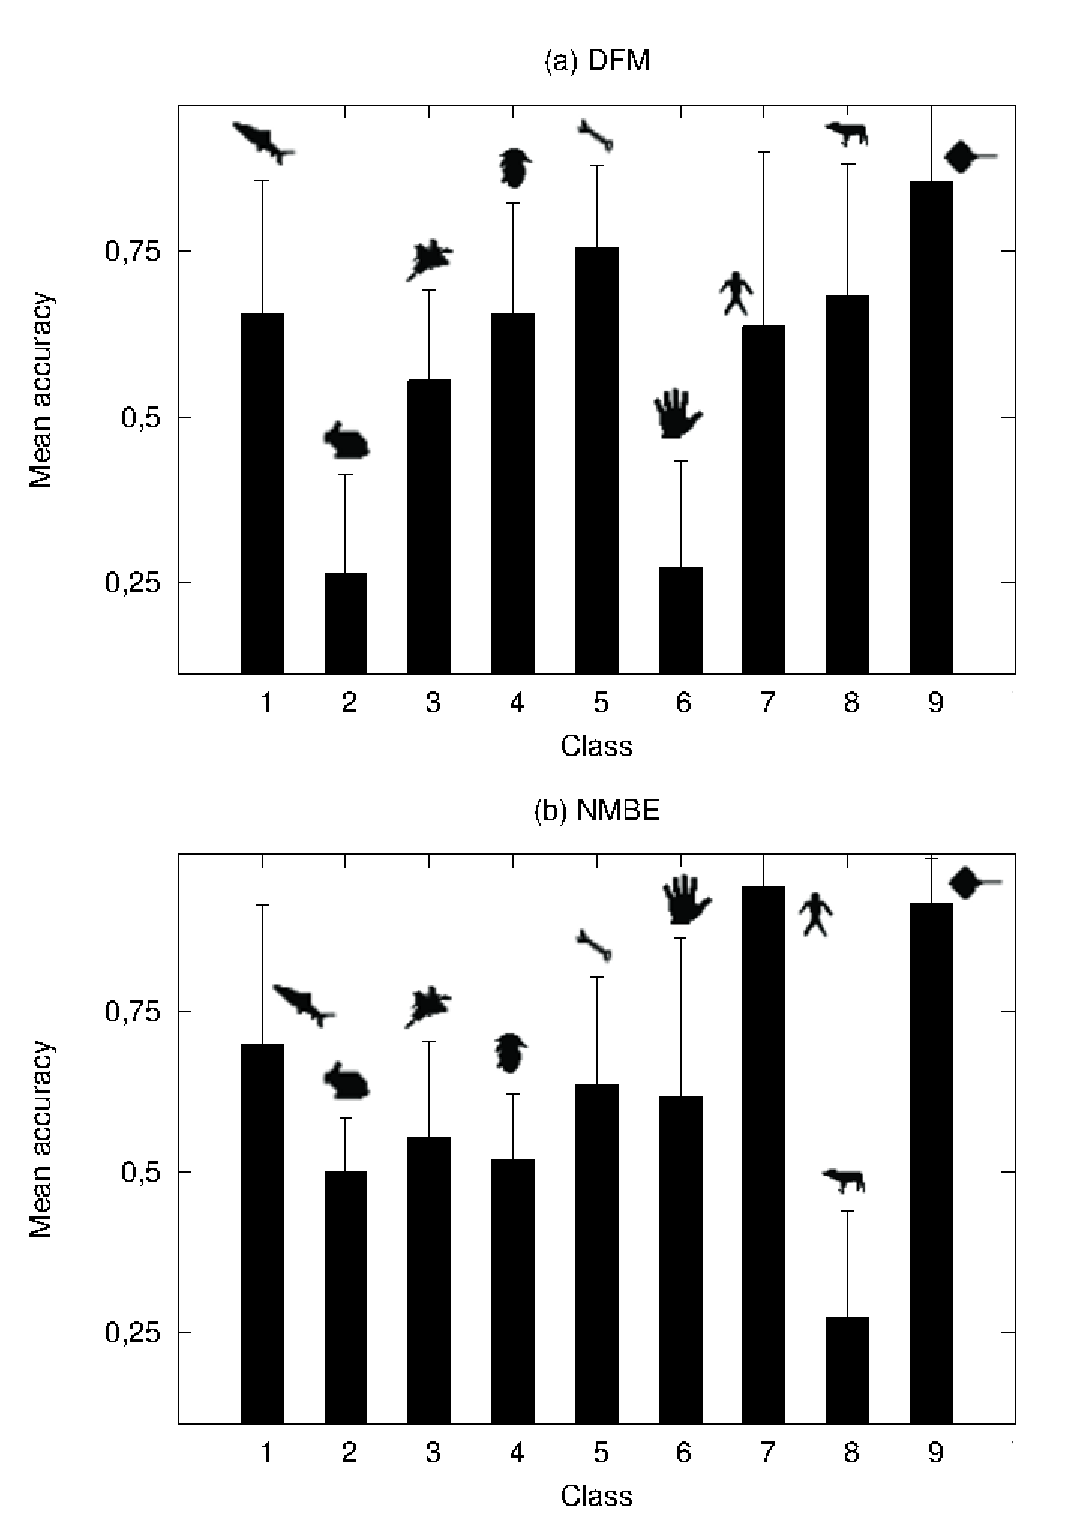
\includegraphics[width=0.75\textwidth]{resultado_acuracia.eps}
\end{figure}

\end{comment}

\color{black}
\begin{comment}
\section{Bases de imagens}
\end{comment}
\begin{comment}
\begin{figure}
\centering
\caption{\label{Met:1}Metodologia 1}
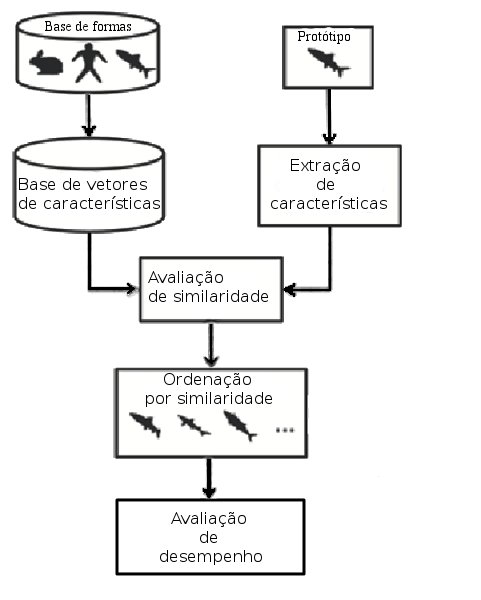
\includegraphics[width=0.5\textwidth]{Metodologia1.eps}
\end{figure}

\begin{figure}
\centering
\caption{\label{Met:2}Metodologia 2}
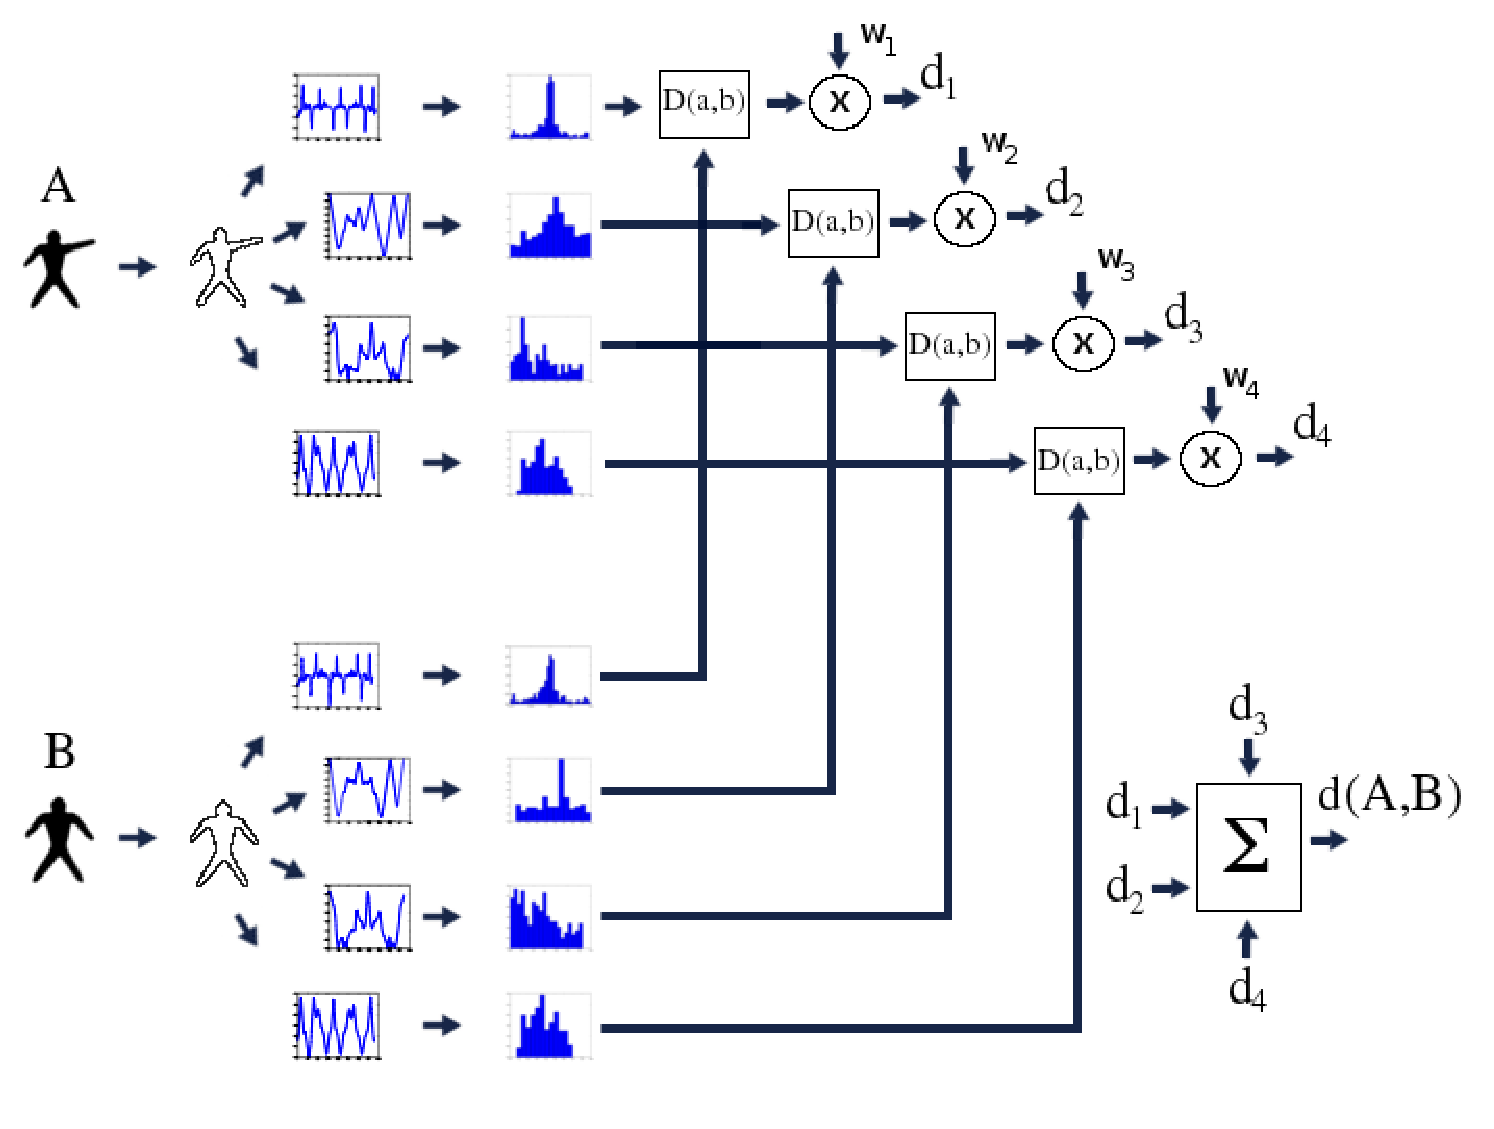
\includegraphics[width=\textwidth]{figura_metodo.eps}
\end{figure}
\end{comment}